\documentclass{article}

\usepackage{geometry}
\usepackage{mathtools}
\usepackage{graphicx}
\usepackage{subcaption}
\usepackage[hidelinks]{hyperref}
\usepackage{cleveref}
\usepackage{tikz}
\usepackage{pgfplots}

\newcommand{\mail}[1]{
  \href{mailto:#1}{#1}
}

\geometry{
  top=2cm,
  bottom=2cm,
  right=3cm,
  left=3cm
}

\pgfplotsset{
  compat=1.13,
  every axis/.prefix style={
    width=.85\textwidth,
    height=200pt,
    legend cell align=left
  },
  every axis plot/.style={
    no marks,
    line width=.8pt
  }
}

\begin{document}

\begin{center}
  \textbf{
    \LARGE Deep Learning with Stacked AEs \& RBMs \\
    \vspace{.5ex}
    \large DD2437 - Artificial Neural Networks \& Deep Architectures - Lab 4\\
    \vspace{1ex}
  }
  \large
  \begin{tabular}{ccc}
    Niels Agerskov & Lukas Bjarre & Gabriel Carrizo \\
    \mail{agerskov@kth.se} & \mail{lbjarre@kth.se} & \mail{gabcar@kth.se}
  \end{tabular}
  \\
  \vspace{.5ex}
  \rule{\textwidth}{0.4pt}
\end{center}

This lab will examine two different artificial neural network structures,
Auto Encoders (AE) and Restricted Boltzmann Machines (RBM).
Their effectiveness in a learning task 
and the effect of the layer depth of the models
will be tested and evaluated.

\section{Feature learning}
In this first task shallow versions of both models are trained
as benchmarks for the later deeper versions.
The dataset used is a subset of the MNIST dataset
containing $28 \times 28$ images of handwritten digits from 0 to 9
together with correct labels of the written digit.
All the pixel values has for simplicity's sake been converted to binary values
via simple thresholding.
A total of 10000 images are used from the dataset,
which has been further subdivided into a training set of size 8000 and a validation set of size 2000.

\subsection{Hidden unit size}
The input size hyperparameter for both of the models is decided by the shape of the data.
In our case we require $28 \times 28 = 784$ input nodes, one for each image pixel.
We do however have a choice in the number of hidden units, $n_{\text{h}}$.

Both models were trained with $n_\text{h} = 50,\,75,\,100,\,150$ hidden units.
The error curves on the validation set during the training are displayed
in \cref{fig:rbmtraining} for the RBM,
and in \cref{fig:aetrainingsgd} for the AE using Stochastic Gradient Descent (SGD).
However, the AE clearly converges to the same values no matter the number of hidden units.
Complementary to using SGD to train the AE ADADELTA was also used,
which error curve can be seen in \cref{fig:aetrainingadadelta}.
ADADELTA shows a similar improvement given more hidden units as the error curves for the RBM.
The errors are also on one order of magnitude smaller compared to the errors using SGD,
which is why the ADADELTA trained AE is only used furthermore.

\begin{figure}[!ht]
  \centering
  \begin{tikzpicture}
    \begin{axis}[
      title=\textbf{RBM training error},
      xlabel={Epoch},
      ylabel={Validation error},
    ]
      \foreach \color/\hiddenunits in {10/50, 40/75, 70/100, 100/150} { 
        \edef\temp{
          \noexpand\addplot +[
            color=red!\color!blue
          ]
          table [
            x index=0,
            y index=2,
            col sep=comma
          ]
          {../data/rbm_hidden_20e_\noexpand\hiddenunits.csv};
          \noexpand\addlegendentry{$n_{\text{h}} = \hiddenunits$}
        }
        \temp
      }
    \end{axis}
  \end{tikzpicture}
  \caption{Error curves on the validation set for the RBM.}
  \label{fig:rbmtraining}
\end{figure}


\begin{figure}[!ht]
  \centering
  \begin{tikzpicture}
    \begin{axis}[
      title=\textbf{AE training error with SGD},
      xlabel={Epoch},
      ylabel={Validation error},
    ]
      \foreach \color/\hiddenunits in {10/50, 40/75, 70/100, 100/150} { 
        \edef\temp{
          \noexpand\addplot +[
            color=red!\color!blue
          ]
          table [
            x index=0,
            y index=2,
            col sep=comma
          ]
          {../data/ae_hidden_150e_\noexpand\hiddenunits.csv};
          \noexpand\addlegendentry{SGD, $n_{\text{h}} = \hiddenunits$}
        }
        \temp
      }
    \end{axis}
  \end{tikzpicture}
  \caption{Error curves on the validation set for the AE using SGD.}
  \label{fig:aetrainingsgd}
\end{figure}

\begin{figure}[!ht]
  \centering
  \begin{tikzpicture}
    \begin{axis}[
      title=\textbf{AE training error with ADADELTA},
      xlabel={Epoch},
      ylabel={Validation error},
    ]
      \foreach \color/\hiddenunits in {10/50, 40/75, 70/100, 100/150} { 
        \edef\temp{
          \noexpand\addplot +[
            color=red!\color!blue
          ]
          table [
            x index=0,
            y index=2,
            col sep=comma
          ]
          {../data/ae_hidden_adadelta_150e_\noexpand\hiddenunits.csv};
          \noexpand\addlegendentry{ADADELTA, $n_{\text{h}} = \hiddenunits$}
        }
        \temp
      } 
    \end{axis}
  \end{tikzpicture}
  \caption{Error curves on the validation set for the AE using ADADELTA.}
  \label{fig:aetrainingadadelta}
\end{figure}

The quality of the models can be seen in \cref{fig:recall},
where one image of each class have been used to get both models recalled versions.
\begin{figure}[!ht]
  \centering
  \begin{subfigure}[t]{\textwidth}
    \centering
    
\includegraphics[width=0.9\textwidth]{../plots/3_1_1/orig_images.png}
    \caption{Input patterns}
    \label{fig:inputpatterns}
  \end{subfigure}
  ~
  \begin{subfigure}[t]{\textwidth}
    \centering
    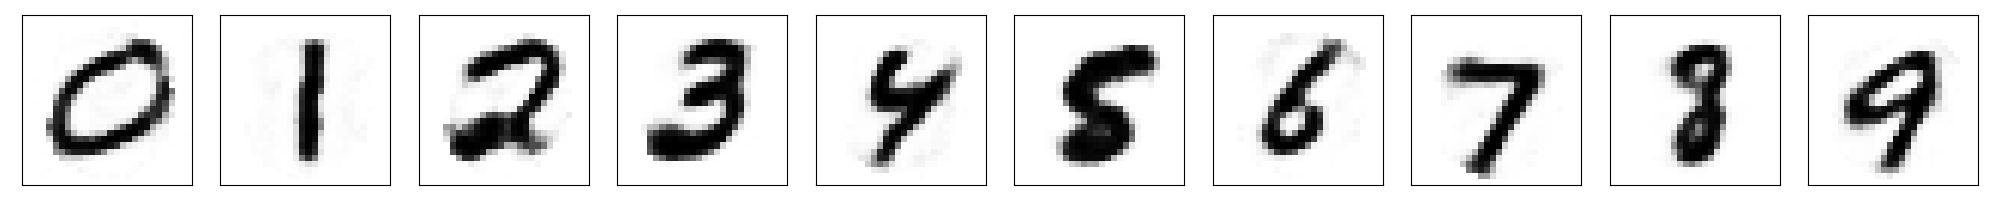
\includegraphics[width=0.9\textwidth]{../plots/3_1_1/recall_ae_h150.png}
    \caption{Recalled patterns of the AE, 150 hidden units}
    \label{fig:recallae}
  \end{subfigure}
  ~
  \begin{subfigure}[t]{\textwidth}
    \centering
    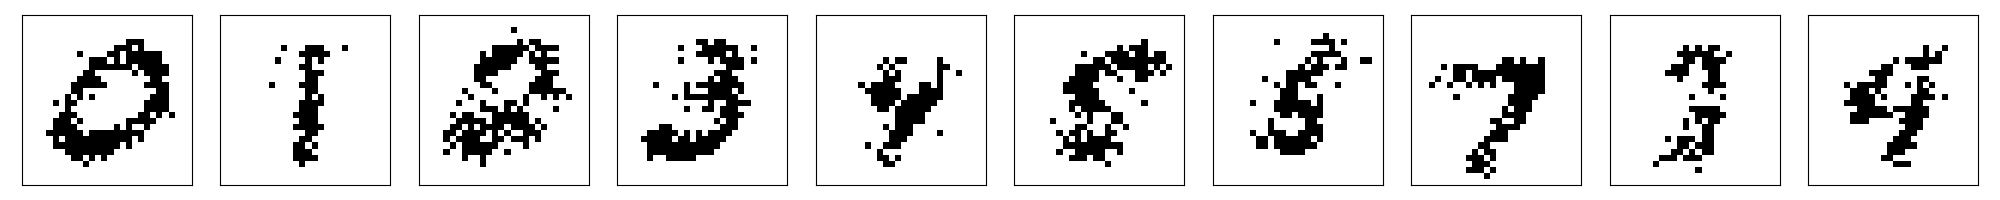
\includegraphics[width=0.9\textwidth]{../plots/3_1_1/recall_rbm_h150.png}
    \caption{Recalled patterns of the RBM, 150 hidden units}
    \label{fig:recallrbm}
  \end{subfigure}
  \caption{Recalled images from the models.}
  \label{fig:recall}
\end{figure}

\subsection{Learned features}
The learned weights of each model can be examined to get an idea what and how the models are learning.
By reshaping the weight vectors back into $28 \times 28$ grids
each hidden units weights can be represented as images
where each pixel value corresponds to the strength of that weight from the given pixel to the hidden unit.
Plots for these are found in \cref{fig:hiddenweights}.
The AE models seems to in general have better trained hidden nodes
as more of the components seems to have learned a specific shape
instead of something that resembles white noise.

\begin{figure}[!ht]
  \centering
  \begin{subfigure}[t]{0.47\textwidth}
    \centering
    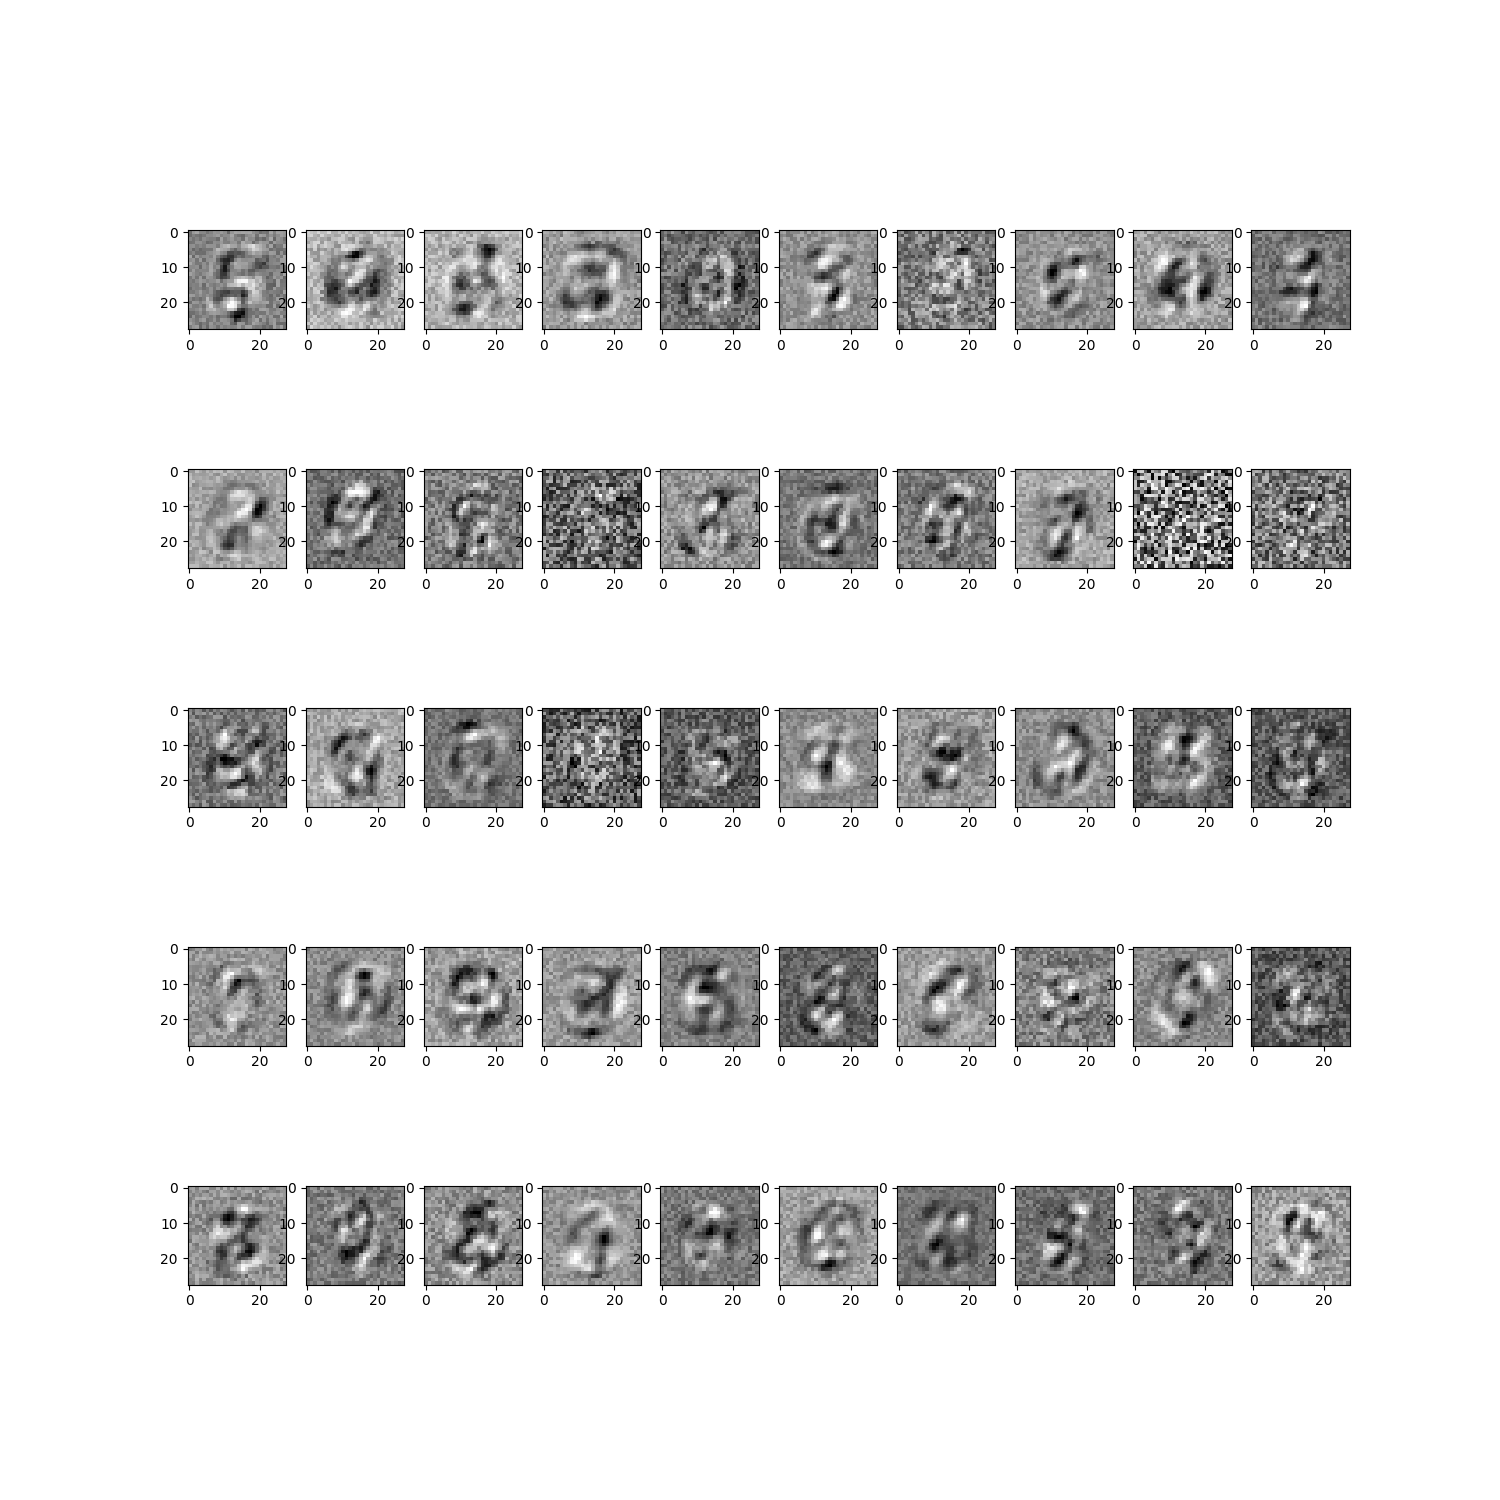
\includegraphics[width=\textwidth]{../plots/3_1_2/last_layer_50_components_100e.png}
    \caption{AE weights, 50 hidden units.}
    \label{fig:w50ae}
  \end{subfigure}
  ~
  \addtocounter{subfigure}{1}
  \begin{subfigure}[t]{0.47\textwidth}
    \centering
    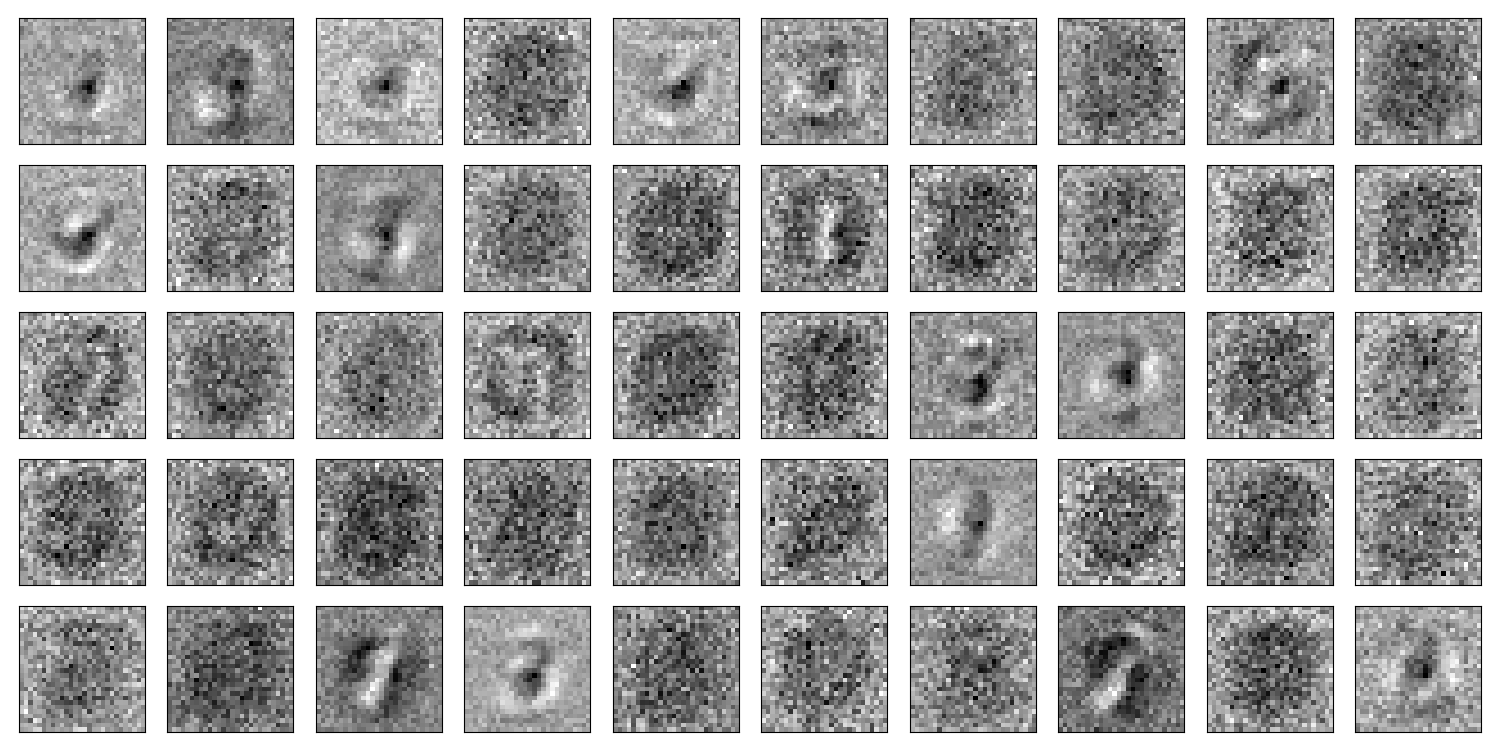
\includegraphics[width=\textwidth]{../plots/3_1_2/rbm_last_layer_50_components_20e.png}
    \caption{RBM weights, 50 hidden units.}
    \label{fig:w50rbm}
  \end{subfigure}
  \addtocounter{subfigure}{-2}
  ~
  \begin{subfigure}[t]{0.47\textwidth}
    \centering
    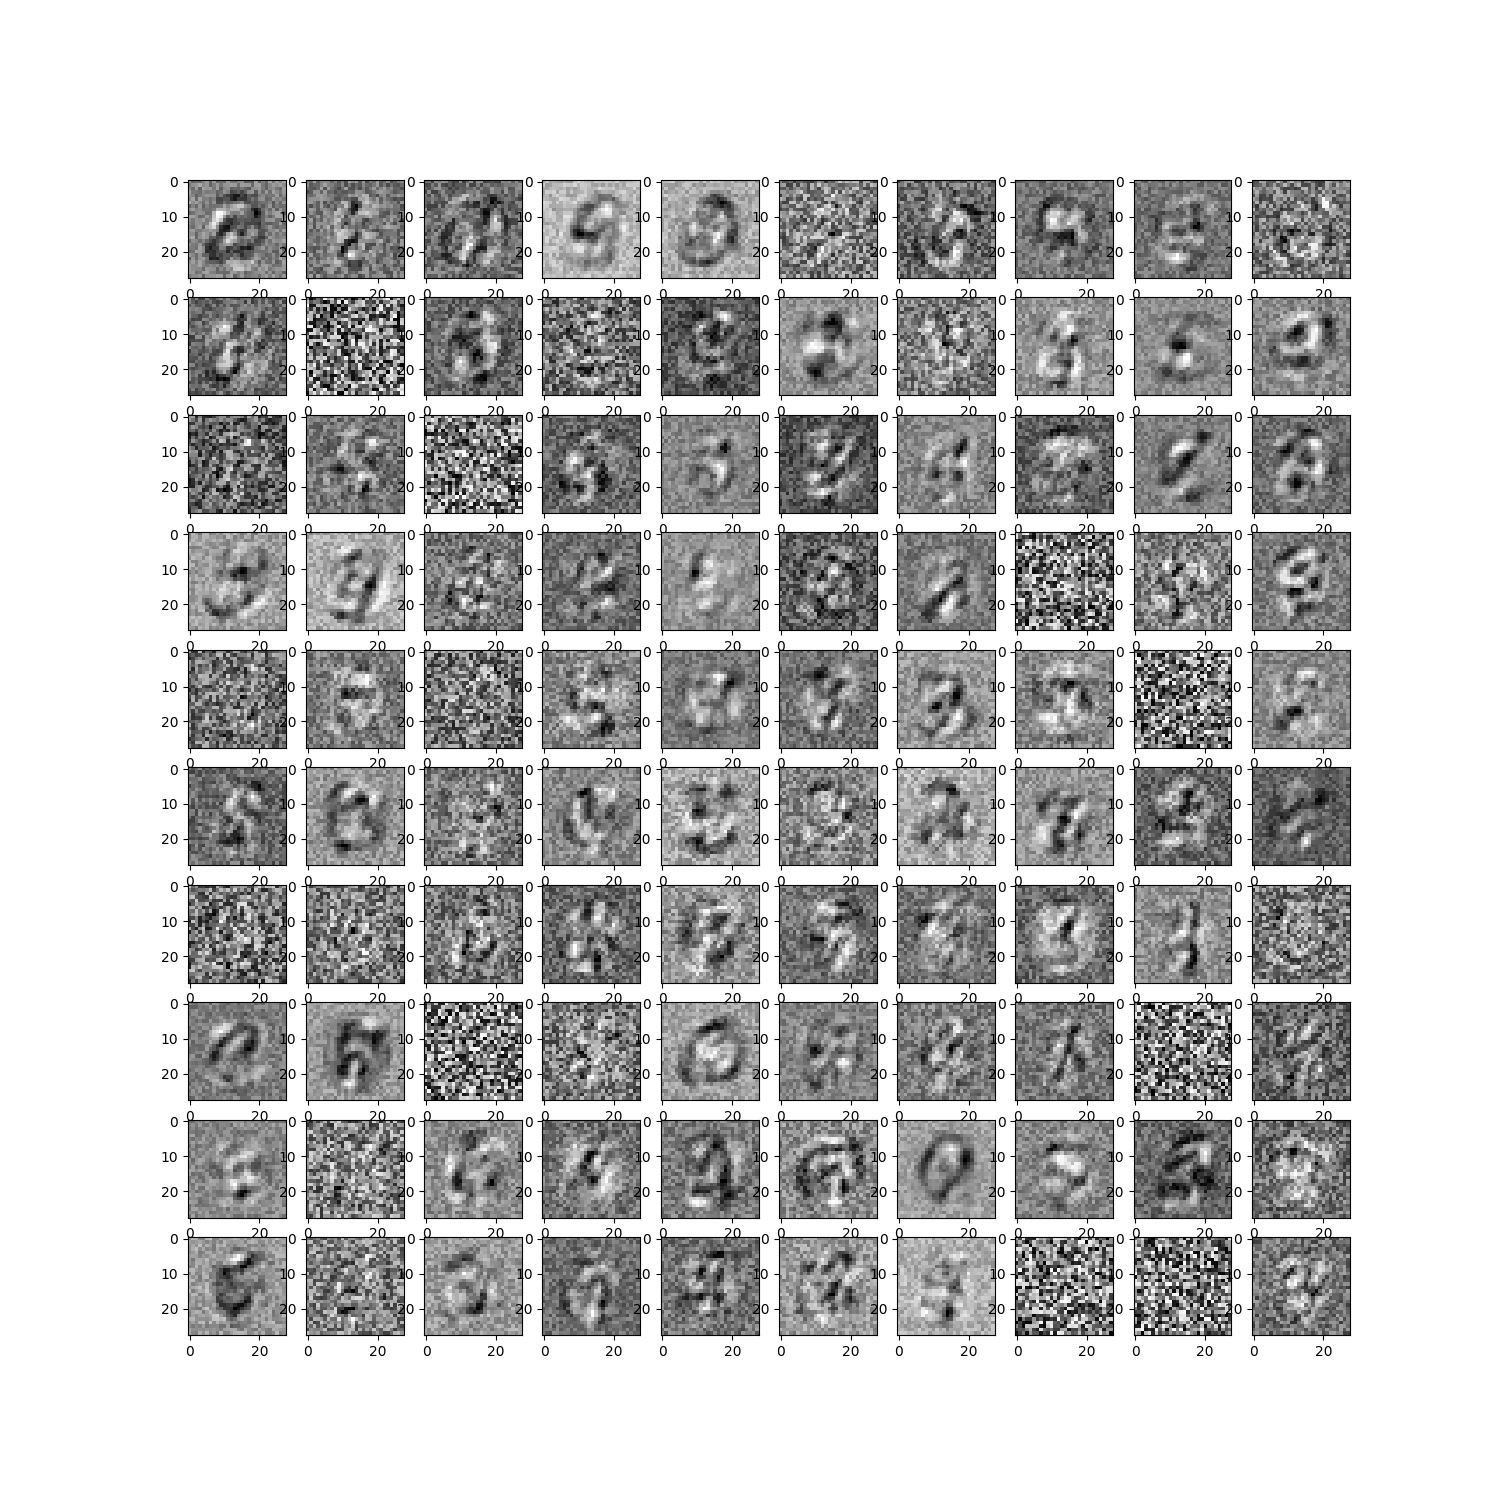
\includegraphics[width=\textwidth]{../plots/3_1_2/last_layer_100_components_100e.png}
    \caption{AE weights, 100 hidden units.}
    \label{fig:w100ae}
  \end{subfigure}
  \addtocounter{subfigure}{1}
  ~
  \begin{subfigure}[t]{0.47\textwidth}
    \centering
    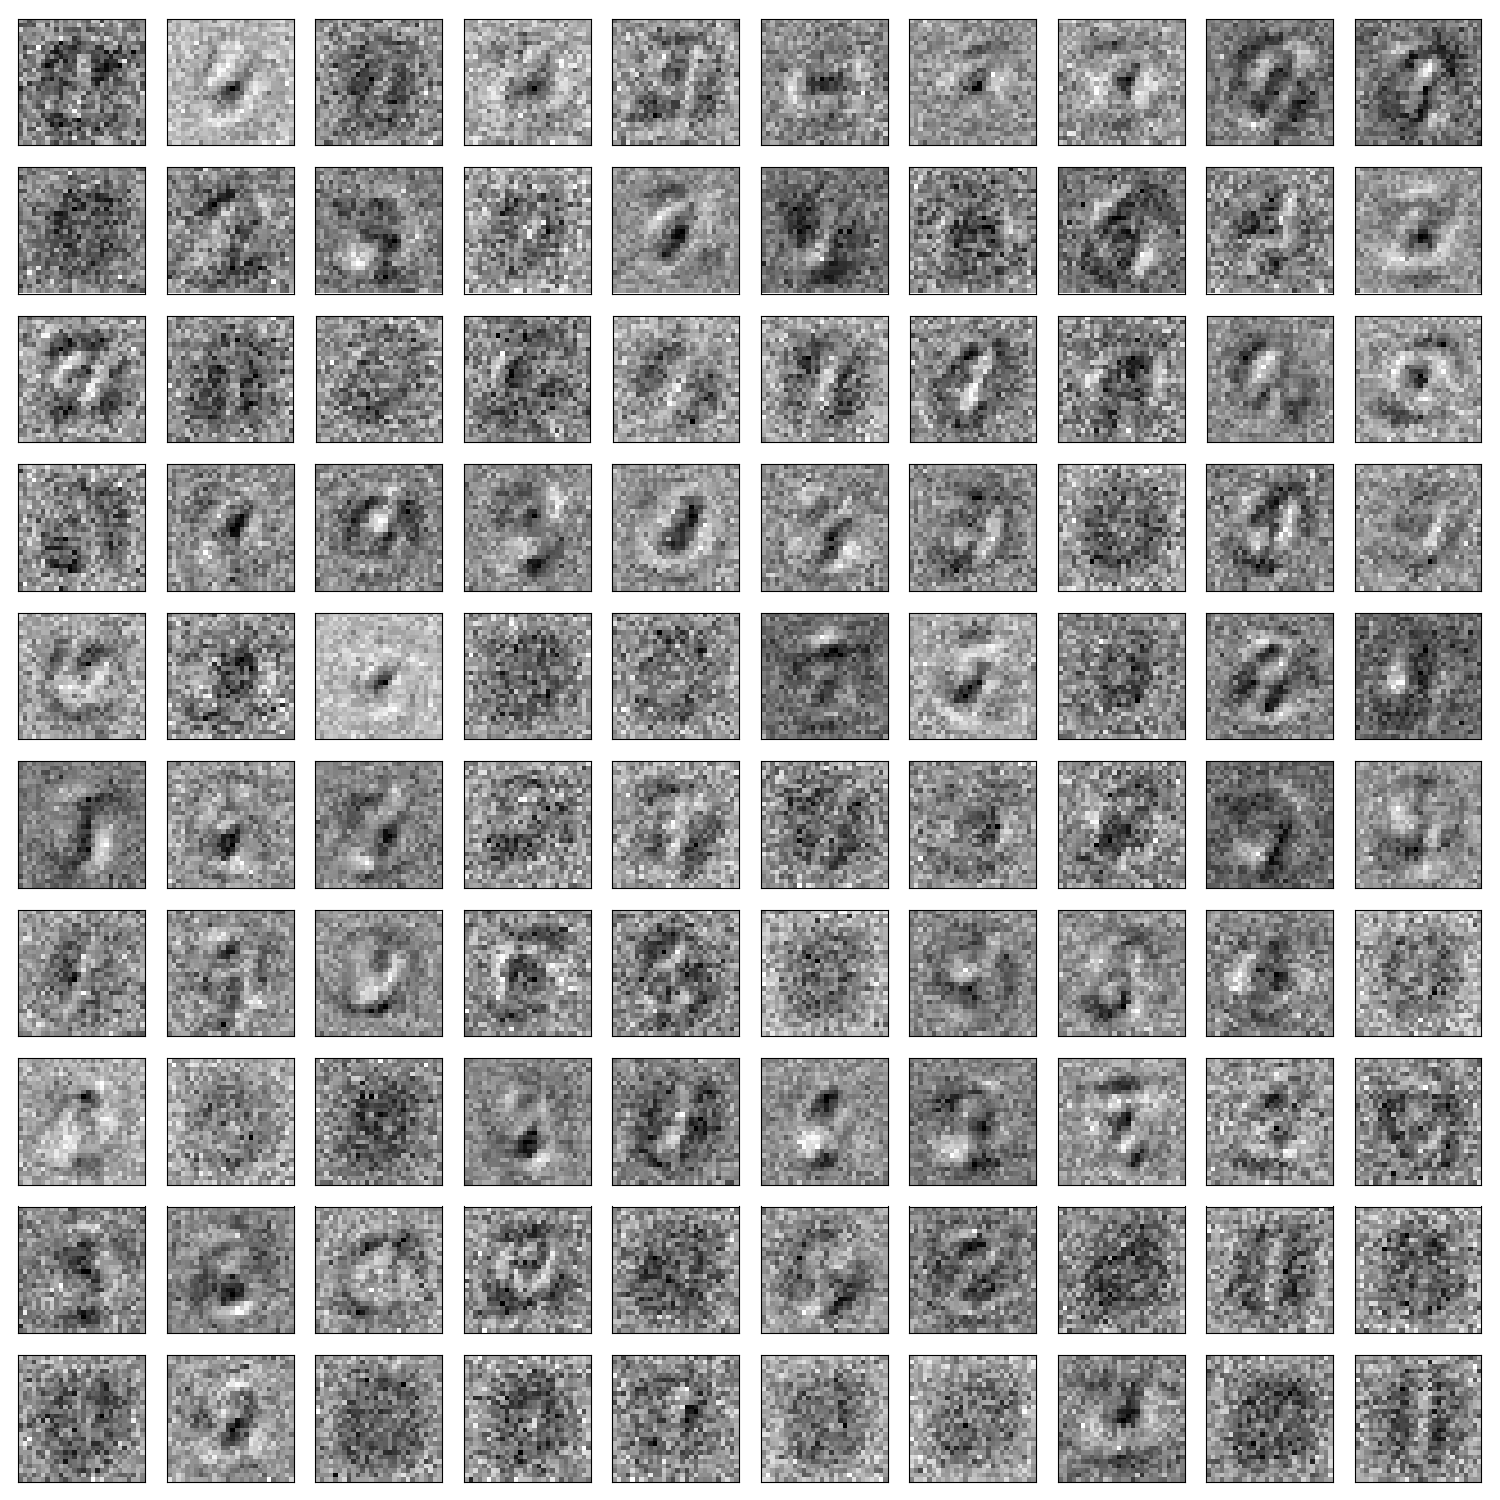
\includegraphics[width=\textwidth]{../plots/3_1_2/rbm_last_layer_100_components_20e.png}
    \caption{RBM weights, 100 hidden units.}
    \label{fig:w100rbm}
  \end{subfigure}
  \caption{
    Image representations of the hidden weights in the AE and RBM models
    for 50 and 100 hidden units.
  }
  \label{fig:hiddenweights}
\end{figure}

\end{document}

